\documentclass[border=3pt,tikz]{standalone}
\usepackage{amsmath}
\usetikzlibrary {3d} 
\usetikzlibrary {arrows}
\usetikzlibrary{shapes.geometric}
\begin{document}
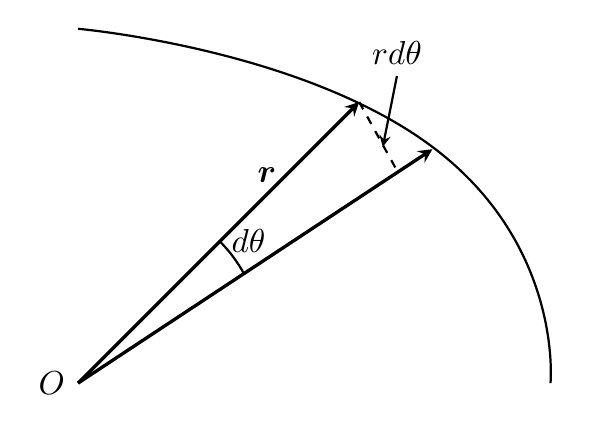
\begin{tikzpicture}[=>stealth, scale=3]
    \draw [black, thick] plot [smooth, tension=1] coordinates { (0,1.5) (1.5,1.0) (2, 0)};
    \draw [black, very thick, -{stealth}] (0, 0) node[left, scale =1.2] {$O$}-- (1.19, 1.19);
    \draw [black, very thick, -{stealth}] (0, 0) -- (1.5, 0.99); 
    \draw [thick] (0.6,0.6) arc (45:29:0.6);
    \node [right, scale=1.2] at (0.6, 0.6) {$d\theta$};
    \node [above, scale=1.2] at (0.8, 0.8) {$\boldsymbol{r}$};
    \draw [thick, dashed] (1.19, 1.19) -- (1.35, 0.9);
    \node [above, scale = 1.2] at (1.35, 1.3) {$r d\theta$ };
    \draw [black, thick, -{stealth}] plot [smooth, tension=1] coordinates { (1.35,1.3) (1.29, 1.0)};
    \end{tikzpicture}
\end{document}